\documentclass{dissert}
\usepackage[T2A]{fontenc}
\usepackage[utf8]{inputenc}
\usepackage[english,russian]{babel}

\usepackage{fullpage}
\usepackage{lastpage}
\usepackage{enumerate}

\usepackage[all]{xy}
% colors
\usepackage{xcolor}
\definecolor{darkgreen}{rgb}{0.0, 0.2, 0.13}
\definecolor{darkcyan}{rgb}{0.0, 0.55, 0.55}

\usepackage{geometry}
\geometry{left=2.5cm}
\geometry{right=1.0cm}
\geometry{top=2.0cm}
\geometry{bottom=2.0cm}
\renewcommand{\baselinestretch}{1.0}

\newcommand{\paragraph}[1]{\noindent\textbf{#1}\quad}


%https://tex.stackexchange.com/questions/163451/total-number-of-citations
\usepackage{totcount}
\newtotcounter{citnum} %From the package documentation
\def\oldbibitem{} \let\oldbibitem=\bibitem
\def\bibitem{\stepcounter{citnum}\oldbibitem}

\makeatletter
\long\def\@makecaption#1#2{%
  \vskip\abovecaptionskip
  \sbox\@tempboxa{#1.~#2}%
  \ifdim \wd\@tempboxa >\hsize
    #1.~#2\par
  \else
    \global \@minipagefalse
    \hb@xt@\hsize{\hfil\box\@tempboxa\hfil}%
  \fi
  \vskip\belowcaptionskip}
\makeatother

\reversemarginpar

\renewcommand{\contentsname}{Содержание}
\renewcommand{\contentsdesc}{Стр.}
\renewcommand{\chaptername}{Глава}

%%% Библиография %%%
\makeatletter
\bibliographystyle{utf8gost71u}     % Оформляем библиографию по ГОСТ 7.1 (ГОСТ Р 7.0.11-2011, 5.6.7)
\makeatother


% Нужные мне пакеты
\usepackage{amsthm}
\usepackage{graphicx}
\usepackage{amssymb}
\usepackage{amsmath}
\usepackage{graphicx}
\usepackage{subfig}
\usepackage{caption}
\usepackage{color}
\usepackage{bm}
\usepackage{tabularx}
\usepackage{url}
\usepackage{multirow}

\newtheorem{theorem}{Теорема}
\newtheorem{lemma}[theorem]{Лемма}
\newtheorem{definition}{Определение}

\usepackage{comment}
\usepackage{rotating}

\usepackage{autonum}

\begin{document}

\begin{titlepage}
%\begin{center}
%\textsc{МОСКОВСКИЙ ФИЗИКО-ТЕХНИЧЕСКИЙ ИНСТИТУТ (ГОСУДАРСТВЕННЫЙ УНИВЕРСИТЕТ)}\\
%\end{center}
%\vspace{1.5cm}
\begin{flushright}
{На правах рукописи}
\end{flushright}
\vspace{1.5cm}
\begin{center}
{Грабовой Андрей Валериевич}
\par
\vspace{2cm}
\textsc{Априорное распределение параметров \\в задачах выбора моделей глубокого обучения}
\par
\vspace{2cm}
{05.13.17~--- Теоретические основы информатики}
\par
\vspace{2cm}
{АВТОРЕФЕРАТ\\
диссертации на соискание ученой степени\\
кандидата физико-математических наук}
\end{center}
\par
\vspace{3.5cm}
\begin{center}
{Москва~--- 2022}
\end{center}
\end{titlepage}

%\clearpage\maketitle
\setcounter{page}{2}
%\pretolerance=10000
%\thispagestyle{empty}
\noindent {Работа выполнена на Кафедре интеллектуальных систем Федерального государственного автономного образовательного учреждения высшего образования <<Московский физико-технический институт (национальный исследовательский институт)>>.

\vspace{0.1cm}

%\begin{sloppy}
%\fontdimen2\font=3pt

\vskip1ex\noindent
\begin{tabularx}{\linewidth}{@{}lX@{}}
  Научный руководитель: & \textbf{Стрижов Вадим Викторович}\\
  & доктор физико-математических наук, Федеральный исследовательский~центр <<Информатика и управление>> Российской академии наук, отдел интеллектуальных систем, ведущий научный сотрудник.
  \\[2pt]
  Официальные оппоненты: & \textbf{???}\\
  & ???\\[2pt]
  & \textbf{???}\\
  & ???
\end{tabularx}
\vskip2ex\noindent

\vspace{0.2cm}
\noindent Защита состоится~???~??? 2022 года~в~??:00 на~заседании диссертационного совета Д 002.073.05 при Федеральном исследовательском центре <<Информатика и управление>> Российской академии наук (ФИЦ~ИУ~РАН) по адресу: 119333, г.\,Москва, ул.\,Вавилова, д.\,40.

\vspace{0.2cm}
\noindent С диссертацией можно ознакомиться в библиотеке Федерального государственного учреждения Федеральный исследовательский центр <<Информатика и управление>> Российской академии наук и на сайте http://www.frccsc.ru/

\vspace{0.2cm}
\noindent Автореферат разослан  \quad \quad ??? 2022 года.

\vspace{0.3cm}
\noindent И. о. ученого секретаря\\
диссертационного совета Д 002.073.05\\
д.т.н.
\hspace{12cm} И. А. Матвеев
}

\clearpage


%%%%%%%%%%%%%%%%%%%%%%%%%%%%%%%%%%%%%%%%%%%%%%%%%%%%%%%%%%%%%%%%%%%%%%%%

\pretolerance=-1

%\setcounter{page}{0}

\section*{Общая характеристика работы}
\textbf{Актуальность темы.}
Построение и выбор оптимальной структуры нейронной сети является вычислительно сложной процедурой~\cite{sutskever2014}, которая значимо влияет на итоговое качество модели. 
При этом большинство параметров модели перестают значимо изменяться уже после небольшого числа итераций алгоритма оптимизации~\cite{Chunyan2016}.
Своевременное определение начала сходимости параметров существенно снижает вычислительные затраты на обучение моделей с большим числом параметров.
Примерами моделей, с большим число параметров, являются AlexNet~\cite{Krizhevsky2012}, VGGNet~\cite{Simonyan2014}, ResNet~\cite{Kaiming2015}, BERT~\cite{Devlin2018, Vaswani2017}, mT5~\cite{Linting2021}, GPT3~\cite{Brown2020}.
Рост числа параметров моделей глубокого обучения влечет снижение интерпретируемости ответов этих моделей~\cite{Ivakhnenko1994}.
Проблема с неинтерпретируемыми моделями рассматривается в классе задач по состязательным атакам~\cite{Zheng2020}.

Проблемой моделей с большим числом параметров является увеличение вычислительной сложности.
Использование избыточно сложных моделей с большим числом неинформативных параметров является препятствием для использования глубоких сетей на мобильных устройствах в режиме реального времени. \textit{Сложность модели} определяется числом настраиваемых параметров модели.
Для снижения числа параметров в литературе рассматривается метод дистилляции модели на основе предсказаний модели учителя~\cite{Hinton2015, Vapnik2015, Lopez2016}.
Сложная модель с большим числом параметров называется~\textit{учитель}. Модель учителя дистиллируется в менее сложную модель с малым числом параметров, которая называется~\textit{ученик}.
Методы дистилляции моделей глубокого обучения введены в работах Дж.\,Е. Хинтона и В.\,Н. Вапником~\cite{Hinton2015, Vapnik2015, Lopez2016}.
Предлагается использовать предсказания модели учителя для повышения качества ученика.
В~\cite{Vapnik2015} В.\,Н. Вапником вводит понятие привилегированной информации. Оно использует дополнительную информацию о данных в момент обучения модели.
Работа~\cite{Lopez2016} объединяет идеи дистилляции~\cite{Hinton2015} с идеями привилегированного обучения~\cite{Vapnik2015}, предложив метод дистилляции учителя в модель ученика в случае, когда признаковое описания объектов не совпадает..
В~\cite{Lopez2016} решается двухэтапная задача. На первом этапе строится модель учителя с расширенным признаковым описанием.
На втором этапе при помощи дистилляции~\cite{Hinton2015} обучается ученика в исходном признаковом описании.
В работе Дж.\,Е. Хинтона~\cite{Hinton2015} поставлены эксперименты по дистилляции моделей глубокого обучения для задачи классификации.
Первый эксперимент анализирует выборку MNIST~\cite{mnist}. Он показывает, что предложенный метод дистилляции позволяет построить нейросетевую модель меньшей сложности на основе модели большей сложности.
Второй эксперимент анализирует метод дистилляции ансамбля моделей в одну нейросетевую модель для решения задачи распознания речи. В работе~\cite{Hinton2015} проводится сравнение дистилляции с моделью смеси экспертов.
Дальнейшие работы по дистилляции моделей глубокого обучения исследуют методы, использующие информации о значениях параметров модели учителя, для оптимизации параметров модели ученика. В~\cite{Zehao2017} предлагается метод передачи селективности~\cite{Tatarchuk2014} нейрона минимизирующий специальную функцию потерь. Эта функция основывается на максимизация среднего описания между выходами слоев модели учителя и модели ученика. В рамках вычислительного эксперимента сравнивалось качество базовой дистилляции с предложенным методов на примере выборок CIFAR~\cite{cifar10} и ImageNet~\cite{imagenet}.

Дистилляция моделей глубокого обучения предполагает, что архитектура модели ученика уже известна. Для выбора архитектуры модели ученика предлагается использовать методы прореживания нейросетевых моделей. В работах~\cite{maclarin2015, luketina2015} предлагается использовать алгоритма градиентного спуска для оптимизации сети. В~\cite{molchanov2017} используются байесовские методы~\cite{neal1995} оптимизации параметров нейронных сетей. Существуют методы поиска оптимальной структуры используя удаления параметров сложной модели~\cite{cun1990, louizos2017, graves2011}. В работе~\cite{cun1990} предлагается удалять наименее~\textit{релевантные} параметры на основе значений первой и второй производных функции ошибки. В~\cite{grabovoy2019} предложен метод определения релевантности параметров аппроксимирующих моделей при помощи метода Белсли. \textit{Релевантность} параметров в работе~\cite{grabovoy2019} определяется на основе ковариационной матрицы параметров модели.
Другим примером задания порядка на множестве параметров служит $l_1$-регуляризация~\cite{Tibshirani1996} и регуляризация ElasticNet~\cite{Hastie2005} для линейных моделей.
Порядок, заданный на множестве значений коэффициентов регуляризации, индуцирует порядок на множестве признаковых описаний и указывает на важность признаков.
В случае нейросетей для регуляризации параметров используется метод исключения параметров~\cite{srivastava2014, molchanov2017}.
Он также задает порядок на множестве параметров модели.

Порядок на множестве параметров нейросети используется не только для удаления неимение релевантных параметров, а и для фиксации параметров в процесе оптимизации параметров. Работа~\cite{grabovoy2020} посвящена оптимизации структуры нейронной сети, а также выбору параметров, которые фиксируются после некоторой итерации градиентного метода. 


\vspace{0.5cm}
\textbf{Цели работы.}
\vspace{0.2cm}
\begin{enumerate}
\item Предложить байесовский метод выбора моделей с использованием модели учителя с привилегированной и накопленной информацией.
\item Предложить метод назначения априорного распределения параметров модели ученика с использованием апостериорного распределения параметров модели учителя.
\item Предложить вероятностную интерпретацию дистилляции моделей глубокого обучения.
\item Предложить метод использования экспертной информации о решаемой задачи прогнозирования при построении априорного распределения параметров.
\item Предложить метод назначения релевантности параметров моделей глубокого обучения для выбора модели машинного обучения.
\end{enumerate}

\vspace{0.5cm}
\textbf{Методы исследования.} Для достижения поставленных целей используются методы вариационного байесовского вывода~\cite{mackay2002,bishop2006}, вероятностные~\cite{shiriyaev1980} методы к анализу моделей глубокого обучения, статистические методы~\cite{kobzar2012,bishop2006} анализа распределений параметров моделей глубокого обучения.

\vspace{0.5cm}
\textbf{Основные положения, выносимые на защиту.}
\vspace{0.3cm}
\begin{enumerate}
    \item Предложен байесовский метод выбора моделей с использованием модели учителя с привилегированной и накопленной информацией.
    \item Доказаны теоремы о свойствах дистилляции, 
    \begin{itemize}
        \item[---] \emph{теоремы об эквивалентности} для дистилляции моделей в случае задачи регрессии и классификации,
        \item[---] \emph{теоремы о виде априорного распределения} параметров модели ученика в байесовской дистилляции.
    \end{itemize}
    \item Предложен метод выравнивания вероятностных пространств параметров. Предложен метод выбора априорного распределения параметров модели ученика с использованием апостериорного распределения параметров модели учителя для случаев
    \begin{itemize}
        \item[---] различных размерностей пространств параметров отдельных слоев,
        \item[---] различного числа слоев нескольких моделей.
    \end{itemize}
    \item Предложены методы задания порядка на множестве параметров моделей
    \begin{itemize}
        \item[---] на основе корреляции параметров,
        \item[---] на основе оценки скорости сходимости параметров.
    \end{itemize}
    \item Предложена вероятностная интерпретации дистилляции моделей глубокого обучения. Исследованы свойства дистилляции моделей глубокого обучения.
\end{enumerate}

\vspace{0.5cm}
\textbf{Научная новизна.} Разработаны новые подходы к назначению априорного распределения параметров моделей. Предложен метод назначения априорного распределения используя экспертную информацию о задаче. Предложены методы задания порядка на множестве параметров нейросетевых моделей на основе анализа мультиколлиниорности параметров и скорости их сходимости. Предложено вероятностное обобщение дистилляции моделей. Предложено байесовское обобщение дистилляции моделей глубокого обобщения.

\vspace{0.5cm}
\textbf{Теоретическая значимость.} Диссертационная работа носит теоретический характер. В работе проводится теоретический анализ методов снижения размерности пространства параметров нейросетевых моделей. Доказаны~\emph{теоремы об эквивалентности} для дистилляции моделей в случае задачи регрессии и классификации. Доказаны~\emph{теоремы об априорном} распределения модели для байесовской дистилляции.

\vspace{0.5cm}
\textbf{Практическая значимость.} Предложенные в работе методы предназначены для построения моделей глубокого обучения в прикладных задачах регрессии и классификации; снижения пространства параметров моделей глубокого обучения; использования экспертной информации для построения моделей; дистилляции параметрических моделей на основе выравнивания архитектур.

\vspace{0.5cm}
\textbf{Степень достоверности и апробация работы.} Достоверность результатов подтверждена математическими доказательствами, экспериментальной проверкой полученных методов на реальных задачах выбора моделей глубокого обучения; публикациями результатов исследования в рецензируемых научных изданиях, в том числе рекомендованных ВАК. Результаты работы докладывались и обсуждались на следующих научных конференциях.
\begin{enumerate}
    \item Задача обучения с экспертом для построения интерпретируемых моделей машинного обучения, Международная конференция <<Интеллектуализация обработки информации>>, 2020.
    \item Привилегированная информация и дистилляция моделей, Всероссийская конференция <<63-я научная конференция МФТИ>>, 2020.
    \item Введение отношения порядка на множестве параметров нейронной сети, Всероссийская конференция <<Математические методы распознавания образов ММРО>>, 2019.
    \item Анализ априорных распределений в задаче смеси экспертов, Всероссийская конференция <<62-я научная конференция МФТИ>>, 2019.
    \item Поиск оптимальной модели при помощи алгоритмов прореживания, Всероссийская конференция <<61-я научная конференция МФТИ>>, 2018.
    \item Автоматическое определение релевантности параметров нейросети, Международная конференция <<Интеллектуализация обработки информации>>, 2018.
\end{enumerate}

Работа поддержана грантами Российского фонда фундаментальных исследований:

\begin{enumerate}
    \item[1)] 19-07-00875, Развитие методов автоматического построения и выбора вероятностных моделей субоптимальной сложности в задачах глубокого обучения,
    \item[2)] 19-07-01155, Развитие теории порождения моделей локальной аппроксимации для классификации сигналов носимых устройств,
    \item[3)] 19-07-00885, Выбор моделей в задачах декодирования временных рядов высокой размерности.
\end{enumerate}

\vspace{0.5cm}
\textbf{Публикации по теме диссертации.} Основные результаты по теме диссертации изложены в 6 печатных изданиях в журналах, рекомендованных ВАК.
\begin{enumerate}
    \item \textit{Грабовой\;А.В., Стрижов\;В.В.} Байесовская дистилляция моделей глубокого обучения~// Автоматика и телемеханика ---~2021. ---~Т.~11. ---~С.~16--29.
    \item \textit{Грабовой\;А.В., Стрижов\;В.В.} Анализ выбора априорного распределения для смеси экспертов~// Журнал вычислительной математики и математической физики ---~2021. ---~Т.~61, №~7. ---~С.~1149--1161.
    \item \textit{Grabovoy\;A., Strijov\;V.} Quasi-periodic time series clustering for human // Lobachevskii Journal of Mathematics ---~2020. Vol.~41. ---~Pp.~333--339.
    \item \textit{Грабовой\;А.В., Бахтеев\;О.Ю., Стрижов\;В.В.} Введение отношения порядка на множестве параметров аппроксимирующих моделей~// Информатика и ее применения ---~2020. ---~Т.~14, №~2. ---~С.~58--65.
    \item \textit{Грабовой\;А.В., Бахтеев\;О.Ю., Стрижов\;В.В.} Определение релевантности параметров нейросети~// Информатика и ее применения ---~2019. ---~Т.~13, №~2. ---~С.~62--70.
    \item \textit{Грабовой\;А.В., Стрижов\;В.В.} Вероятностная интерпретация задачи дистилляции~// Автоматика и телемеханика ---~2022. ---~Т.~1. ---~С.~150--168.
\end{enumerate}

\vspace{0.5cm}
\textbf{Личный вклад.} Все приведенные результаты, кроме отдельно оговоренных случаев, получены диссертантом лично при научном руководстве д.ф.-м.н. В. В. Стрижова.

\vspace{0.5cm}
\textbf{Структура и объем работы.} Диссертация состоит из оглавления, введения, шести разделов, заключения, списка иллюстраций, списка таблиц, перечня основных обозначений и списка литературы из~$99$ наименований. Основной текст занимает~$124$ страницы.

\section*{Основное содержание работы}
Во~\textbf{введении} обоснована актуальность диссертационной работы, сформулированы цели и методы исследования, поставлены основные задачи, обоснована научная новизна, теоретическая и практическая значимость полученных результатов.

В~\textbf{главе~1} рассматривается формальная постановка задачи дистилляции, а также методов выбора априорного распределения параметров.
При построении модели машинного обучения оптимизируются два критерия: сложность модели и точность аппроксимации модели.
\begin{definition}
Сложность модели (структурная сложность)~--- число обучаемых параметров, используемых предсказтельнной моделью.
\end{definition}

\begin{definition}
Дистилляция модели --- снижение сложности модели путем выбора модели в множестве более простых моделей на основе анализа пространства параметров и предсказаний целевой переменной более сложной фиксированной модели.
\end{definition}

\begin{definition}
Привилегированная информация --- множество признаков, доступных только при выборе модели, но не в при тестировании.
\end{definition}

\begin{definition}
Учитель --- фиксированная модель, ответы которой используются при выборе модели ученика.
\end{definition}

\begin{definition}
Ученик --- модель, которая выбирается согласно заданного критерия качества использующего учителя.
\end{definition}

Важным свойством дистиллированных является то, что избыточная сложность модели учителя заключается в большом числе не релевантных параметров.
\begin{definition}
Релевантность параметров --- численная характеристика описывающая влияние параметров на предсказания моделей.
\end{definition}
Предлагается удалять наименее релевантные параметры модели.

Пусть на множестве признаков задана функция учителя $\mathbf{f}\bigr(\mathbf{x}\bigr)$:
\[
\begin{aligned}
\mathbf{f}:\mathbb{R}^{n} \to \mathbb{Y}^*,
\end{aligned}
\]
где $\mathbb{Y}^*=\mathbb{Y}$ для задачи регрессии и $\mathbb{Y}^*$ является единичным симплексом $\mathcal{S}_R$ в пространстве размерности $R$ для задачи классификации. Модель учителя $\mathbf{f}$ ставит объекты $\mathbf{X}$ в соответствие объектам $\mathbf{S},$ то есть  $\mathbf{f}\bigr(\mathbf{x}_i\bigr)=\mathbf{s}_i$.

Требуется выбрать модель ученика $\mathbf{g}\bigr(\mathbf{x}\bigr)$ из множества:
\[
\label{eq:st:G}
\begin{aligned}
\mathfrak{G} = \left\{\mathbf{g}| \mathbf{g}:\mathbb{R}^{n} \to \mathbb{Y}^*\right\},
\end{aligned}
\]
например для задачи классификации множество $\mathfrak{G}$ может быть параметрическим семейством функций линейных моделей:
\[
\label{eq:st:G:lin:cl}
\begin{aligned}
\mathfrak{G}_\text{lin,cl} = \left\{\mathbf{g}\bigr(\mathbf{W}, \mathbf{x}\bigr)| \mathbf{g}\bigr(\mathbf{W}, \mathbf{x}\bigr) = \textbf{softmax}\bigr(\mathbf{W}\mathbf{x}\bigr), \quad \mathbf{W} \in \mathbb{R}^{n\times R}\right\}.
\end{aligned}
\]

Решается задача классификации вида:
\[
    \mathfrak{D} = \{\left(\mathbf{x}_i, y_i\right)\}_{i=1}^{m}, \qquad \mathbf{x}_i \in \mathbb{R}^{n}, \quad y_i \in \mathbb{Y}=\{1, \ldots, R\},
\]
где $y_i$ --- это класс объекта, также обозначим $\mathbf{y}_i$ вектором вероятности для класса $y_i$.

В постановке Хинтона рассматривается параметрическое семейство функций:
\[
\label{eq:G:set:cl}
\mathfrak{G}_{\text{cl}} = \left\{\mathbf{g}| \mathbf{g} = \text{softmax}\bigr(\mathbf{z}\bigr(\mathbf{x}\bigr)/T\bigr), \quad \mathbf{z}: \mathbb{R}^n \to \mathbb{R}^R \right\},
\]
где $\mathbf{z}$ --- это дифференцируемая параметрическая функция заданной структуры, $T$ --- параметр температуры. В качестве модели учителя $\mathbf{f}$ рассматривается функция из множества $\mathfrak{F}_{\text{cl}}$:
\[
\label{eq:F:set:cl}
\mathfrak{F}_{\text{cl}} = \left\{\mathbf{f}| \mathbf{f} = \text{softmax}\bigr(\mathbf{v}\bigr(\mathbf{x}\bigr)/T\bigr), \quad \mathbf{v}: \mathbb{R}^n \to \mathbb{R}^R \right\},
\]
где $\mathbf{v}$ --- это дифференцируемая параметрическая функция заданной структуры, $T$ --- параметр температуры.
Параметр температуры $T$ имеет свойства:
\begin{enumerate}
    \item при $T\to 0$ получаем вектор, в котором один из классов имеет единичную вероятность;
    \item при $T\to \infty$ получаем равновероятные классы.
\end{enumerate}

Функция потерь $\mathcal{L}$ учитывает перенос информации от модели учителя $\mathbf{f}$ к модели ученика $\mathbf{g}$ имеет вид:
\[
\label{eq:hinton:1}
\begin{aligned}
   \mathcal{L}_{st}\bigr(\mathbf{g}\bigr) = &-\sum_{i=1}^{m}\underbrace{{\sum_{r=1}^{R}y^r_i\log\mathbf{g}\bigr(\mathbf{x}_i\bigr)\bigr|_{T=1}}}_{\text{исходная функция потерь}}\\
   &-\sum_{i=1}^{m}\underbrace{{\sum_{r=1}^{R}\mathbf{f}\bigr(\mathbf{x}_i\bigr)\bigr|_{T=T_0}\log\mathbf{g}\bigr(\mathbf{x}_i\bigr)\bigr|_{T=T_0}}}_{\text{слагаемое дистилляция}},
\end{aligned}
\]
где $\cdot\bigr|_{T=t}$ обозначает, что параметр температуры $T$ в предыдущей функции равняется $t$.

Получаем оптимизационную задачу:
\[
\label{eq:hinton:opt}
\begin{aligned}
   \hat{\mathbf{g}} = \arg\min_{\mathbf{g} \in \mathfrak{G}_{\text{cl}}} \mathcal{L}_{st}\bigr(\mathbf{g}\bigr).
\end{aligned}
\]

Для задачи назначения релевантности параметров ...

В~\textbf{главе~2} рассматривается вероятностное обоснование метода дистилляции моделей глубокого обучения.

Задано распределение целевой переменной~$p\bigr(\mathbf{y}_i|\mathbf{x}_i, \mathbf{g}\bigr)$.
Для поиска~$\hat{\mathbf{g}}$ воспользуемся методом максимального правдоподобия. В качестве~$\hat{\mathbf{g}}$ выбирается функция, которая максимизирует правдоподобие модели:
\begin{gather}
\label{ch-2:eq:st:7}
\begin{aligned}
\hat{\mathbf{g}} = \arg\max_{\mathbf{g}\in \mathfrak{G}} \prod_{i=1}^{N}p\bigr(\mathbf{y}_{i}|\mathbf{x}_i, \mathbf{g}\bigr),
\end{aligned}
\end{gather}
где множество~$\mathfrak{G}$ задается~в~\eqref{eq:st:G}.
\section{Подход дистилляции модели учителя в модель ученика}
Рассмотрим вероятностную постановку, в которой выполнены ограничения:
\begin{enumerate}[1)]
	\item задано распределение целевой переменной~$p\bigr(\mathbf{y}_i|\mathbf{x}_i, \mathbf{g}\bigr)$;
	\item задано совместное распределение целевой переменной и ответов модели учителя~$p\bigr(\mathbf{y}_i, \mathbf{s}_i|\mathbf{x}_i, \mathbf{g}\bigr)$;
	\item для всех $\omega \in \bm{\Omega}^*$ элементы $\mathbf{y}(\omega)$ и $\mathbf{s}(\omega)$ являются зависимыми величинами, так как ответы учителя должны коррелировать с истинными ответами;
	\item если $|\bm{\Omega}^*|=0$, то решение должно соответствовать решению~\eqref{ch-2:eq:st:7}.
\end{enumerate}

Рассмотрим совместное правдоподобие истинных меток и меток учителя:
\begin{gather}
\label{eq:st:8}
\begin{aligned}
p\bigr(\mathbf{Y}, \mathbf{S}|\mathbf{X}, \mathbf{g}, \mathcal{I}\bigr)=\prod_{i\not\in \mathcal{I}}p\bigr(\mathbf{y}_i|\mathbf{x}_i, \mathbf{g}\bigr)\prod_{i\in \mathcal{I}}p\bigr(\mathbf{y}_i, \mathbf{s}_i|\mathbf{x}_i, \mathbf{g}\bigr).
\end{aligned}
\end{gather}
Перепишем~$p\bigr(\mathbf{y}_i, \mathbf{s}_i|\mathbf{x}_i, \mathbf{g}\bigr)$ по формуле условной вероятности:
\begin{gather}
\label{eq:st:bernuli}
\begin{aligned}
p\bigr(\mathbf{y}_i, \mathbf{s}_i|\mathbf{x}_i, \mathbf{g}\bigr) = p\bigr(\mathbf{y}_i|\mathbf{x}_i, \mathbf{g}\bigr)p\bigr(\mathbf{s}_i|\mathbf{y}_i, \mathbf{x}_i, \mathbf{g}\bigr).
\end{aligned}
\end{gather}
Подставляя выражения~\eqref{eq:st:bernuli} в~\eqref{eq:st:8}, получим
\begin{gather}
\label{eq:st:9}
\begin{aligned}
p\bigr(\mathbf{Y}, \mathbf{S}|\mathbf{X}, \mathbf{g}, \mathcal{I}\bigr)=\prod_{i\not\in \mathcal{I}}p\bigr(\mathbf{y}_i|\mathbf{x}_i, \mathbf{g}\bigr)\prod_{i\in \mathcal{I}}p\bigr(\mathbf{y}_i|\mathbf{x}_i, \mathbf{g}\bigr)\prod_{i\in \mathcal{I}}p\bigr(\mathbf{s}_i|\mathbf{y}_i, \mathbf{x}_i, \mathbf{g}\bigr).
\end{aligned}
\end{gather}
Заметим, что~$\mathbf{y}_i$ и~$\mathbf{s}_i$ зависимы только через переменную~$\mathbf{x}_i$, тогда~$p\bigr(\mathbf{s}_i|\mathbf{y}_i, \mathbf{x}_i, \mathbf{g}\bigr)=p\bigr(\mathbf{s}_i|\mathbf{x}_i, \mathbf{g}\bigr)$. Получаем совместное правдоподобие
\begin{gather}
\label{eq:st:10}
\begin{aligned}
p\bigr(\mathbf{Y}, \mathbf{S}|\mathbf{X}, \mathbf{g}, \mathcal{I}\bigr)=\prod_{i\not\in \mathcal{I}}p\bigr(\mathbf{y}_i|\mathbf{x}_i, \mathbf{g}\bigr)\prod_{i\in \mathcal{I}}p\bigr(\mathbf{y}_i|\mathbf{x}_i, \mathbf{g}\bigr)\prod_{i\in \mathcal{I}}p\bigr(\mathbf{s}_i|\mathbf{x}_i, \mathbf{g}\bigr).
\end{aligned}
\end{gather}
Используя~\eqref{eq:st:10}, получаем оптимизационную задачу для поиска~$\hat{\mathbf{g}}$
\begin{gather}
\label{eq:st:11}
\begin{aligned}
\hat{\mathbf{g}} = \arg\max_{\mathbf{g}\in \mathcal{G}} \prod_{i\not\in \mathcal{I}}p\bigr(\mathbf{y}_i|\mathbf{x}_i, \mathbf{g}\bigr)\prod_{i\in \mathcal{I}}p\bigr(\mathbf{y}_i|\mathbf{x}_i, \mathbf{g}\bigr)\prod_{i\in \mathcal{I}}p\bigr(\mathbf{s}_i|\mathbf{x}_i, \mathbf{g}\bigr).
\end{aligned}
\end{gather}
Для удобства минимизируется логарифм выражения. Тогда из~\eqref{eq:st:11} получаем, что
\begin{gather}
\label{eq:st:12}
\begin{aligned}
\hat{\mathbf{g}} = \arg\max_{\mathbf{g}\in \mathcal{G}} \sum_{i\not\in \mathcal{I}}\log p\bigr(\mathbf{y}_i|\mathbf{x}_i, \mathbf{g}\bigr) + \left(1-\lambda\right)\sum_{i\in \mathcal{I}}\log p\bigr(\mathbf{y}_i|\mathbf{x}_i, \mathbf{g}\bigr) + \lambda\sum_{i\in \mathcal{I}}\log p\bigr(\mathbf{s}_i|\mathbf{x}_i, \mathbf{g}\bigr),
\end{aligned}
\end{gather}
где параметр~$\lambda \in [0,1]$ введен для взвешивания ошибок на истинных ответах и ошибок ответов учителя.

На рис.~\ref{fg:st:plate} показан вид вероятностной модели в графовой нотации для произвольной функции~$\mathbf{g}$.

\begin{figure}[!ht]\center
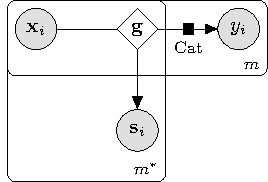
\includegraphics[width=0.35\textwidth]{results/privlearn/general_model}
\caption{Вероятностная модель в графовой нотации.}
\label{fg:st:plate}
\end{figure}

Для каждой реализации~$\mathbf{g}$ соответствующий блок требует уточнения. На рис.~\ref{fg:ex:synt:plate} показана более подробная реализация в случае, когда~$\mathbf{g}$~--- линейная модель.

\paragraph{Классификация.} Для задачи многоклассовой классификации рассматриваются вероятностные 
{\sl{п\,р\,е\,д\,п\,о\,л\,о\,ж\,е\,н\,и\,я:}}
\begin{enumerate}[1)]
\label{st:class:1}
	\item \emph{рассматривается функция учителя} $\mathbf{f}\in\mathfrak{F}_{\text{cl}}^{*}$~\emph{\eqref{eq:F:set:cl:priv};}
	\item \emph{рассматривается функция ученика}   $\mathbf{g}\in\mathfrak{G}_{\text{cl}}$~\emph{\eqref{eq:G:set:cl};}
	\item \emph{для истинных меток рассматривается категориальное распределение}~$p\bigr(y|\mathbf{x}, \mathbf{g}\bigr) = \text{Cat}\bigr(\mathbf{g}\bigr(\mathbf{x}\bigr)\bigr)$, \emph{где $\mathbf{g}\bigr(\mathbf{x}\bigr)$ задает вероятность каждого класса;}
	\item \emph{для меток учителя введем плотность распределения}
\begin{gather}
\label{reg:dist}
\begin{aligned}
	p\bigr(\mathbf{s}|\mathbf{x}, \mathbf{g}\bigr) = C\prod_{r=1}^{R}g_r\bigr(\mathbf{x}\bigr)^{s^r},
\end{aligned}
\end{gather}
\emph{где~$g^r$~--- вероятность класса~$r$, которую предсказывает модель ученика, а~$s^r$~--- вероятность класса~$r$, которую предсказывает модель учителя.}
\end{enumerate}
\begin{theorem}
\label{theorem:st:dist}
Пусть вероятность каждого класса отделима от нуля и единицы, т.е. для всех~$r$ выполняется условие
\[1 > 1- \varepsilon > g_r\bigr(\mathbf{x}\bigr) > \varepsilon > 0.
\]

Тогда при
\begin{gather}
C=\left(-1\right)^{R}\frac{R^{R/2}}{2^{R(R-1)/2}}\prod_{r=1}^{R}g_r\bigr(\mathbf{x}\bigr)\log g_r\bigr(\mathbf{x}\bigr)
\end{gather}
функция $p\bigr(\mathbf{s}|\mathbf{x}, \mathbf{g}\bigr)$, определенная в~\eqref{reg:dist}, является плотностью распределения.
\end{theorem}
\begin{proof}
	Во-первых, покажем, что для произвольного вектора ответов $\mathbf{s} \in \mathcal{S}_R$ выполняется $p\bigr(\mathbf{s}|\mathbf{x}, \mathbf{g}\bigr) \geq 0$. Заметим, что для всех~$r$ выполняется
	\[\log g_r\bigr(\mathbf{x}\bigr) < 0,\] тогда
\begin{gather}
\begin{aligned}
	C=\underbrace{\frac{R^{R/2}}{2^{R(R-1)/2}}}_{>0}\prod_{r=1}^{R}\underbrace{g_r\bigr(\mathbf{x}\bigr)}_{>\varepsilon}\underbrace{\left(-\log g_r\bigr(\mathbf{x}\bigr)\right)}_{>0} > 0.
\end{aligned}
\end{gather}
Так как~$g_r\bigr(\mathbf{x}\bigr) >0$ и~$C>0$, получаем, что $p\bigr(\mathbf{s}|\mathbf{x}, \mathbf{g}\bigr) \geq 0$.
	Во-вторых, покажем, что интеграл по всему пространству ответов~$\mathcal{S}_R$ является конечным:
	\begin{gather}
	\label{theorem:st:dist:eq:1}
	\begin{aligned}
		\int\limits_{\mathcal{S}_R}&p\bigr(\mathbf{s}|\mathbf{x}, \mathbf{g}\bigr)ds = \int\limits_{\mathcal{S}_R}\prod_{r=1}^{R}g_r\bigr(\mathbf{x}\bigr)^{s^r}ds = \prod_{r=1}^{R}\int\limits_{\mathcal{S}_R}g_r\bigr(\mathbf{x}\bigr)^{s^r}ds =\\ 
		& = \prod_{r=1}^{R}\int\limits_{0}^{1}\frac{r^{R-1}\sqrt{R}}{\left(R-1\right)!\sqrt{2^{R-1}}}g_r\bigr(\mathbf{x}\bigr)^{r}dr = \prod_{r=1}^{R}\underbrace{\frac{\sqrt{R}}{\left(R-1\right)!\sqrt{2^{R-1}}}}_{D}\int\limits_{0}^{1}r^{R-1}g_r\bigr(\mathbf{x}\bigr)^{r}dr =\\
		& = D^R\prod_{r=1}^{R} \int\limits_{0}^{1}r^{R-1}\exp\bigr(r\log g_r\bigr(\mathbf{x}\bigr)\bigr)dr =\\
		& = \left(-D\right)^R\prod_{r=1}^{R}\log g_r\bigr(\mathbf{x}\bigr)\left(\Gamma\bigr(R\bigr) - \Gamma\bigr(R, -\log g_r\bigr(\mathbf{x}\bigr)\bigr)\right) =\\
		& = \left(-D\right)^R\left(R-1\right)!^R\prod_{r=1}^{R}\log g_r\bigr(\mathbf{x}\bigr)\left(1 -g_r\bigr(\mathbf{x}\bigr) \exp_{R-1}\bigr(-\log g_r\bigr(\mathbf{x}\bigr)\bigr)+g_r\bigr(\mathbf{x}\bigr)\right) =\\
		& = \frac{\left(-\sqrt{R}\right)^R}{2^{R(R-1)/2}}\prod_{r=1}^{R}\log g_r\bigr(\mathbf{x}\bigr)\left(1 -g_r\bigr(\mathbf{x}\bigr) \exp_{R-1}\bigr(-\log g_r\bigr(\mathbf{x}\bigr)\bigr)+g_r\bigr(\mathbf{x}\bigr)\right) < \infty,
	\end{aligned}
	\end{gather}
где~$\Gamma\bigr(R\bigr)$ является гамма-функцией, $\Gamma\bigr(R, -\log g_r\bigr(\mathbf{x}\bigr)\bigr)$ является неполной гамма функцией, $\exp_{r}\bigr(x\bigr)$ является суммой Тейлора из первых~$r$ слагаемых. В рамках приближенных расчетов считается, что $\exp_{r}\bigr(x\bigr)\approx\exp\bigr(x\bigr),$ тогда с учетом~\eqref{theorem:st:dist:eq:1} получаем
	\begin{gather}
	\label{theorem:st:dist:eq:2}
	\begin{aligned}
		C\bigr(\mathbf{g}, \mathbf{x}\bigr) = \int\limits_{\mathcal{S}_R}p\bigr(\mathbf{s}|\mathbf{x}, \mathbf{g}\bigr)ds \approx \left(-1\right)^{R}\frac{R^{R/2}}{2^{R(R-1)/2}}\prod_{r=1}^{R}g_r\bigr(\mathbf{x}\bigr)\log g_r\bigr(\mathbf{x}\bigr).
	\end{aligned}
	\end{gather}
Полученное выражение~\eqref{theorem:st:dist:eq:2} заканчивает доказательство теоремы~1.
\end{proof}

Из теоремы~\ref{theorem:st:dist} следует, что плотность, введенная для меток учителя, является плотностью распределения. Поэтому можно воспользоваться выражением~\eqref{eq:st:12}.
Используя предположения 1--4 и подставляя в~\eqref{eq:st:12}, получаем  оптимизационную задачу:
\begin{gather}
\label{eq:st:class:1}
\begin{aligned}
\hat{\mathbf{g}} = \arg\max_{\mathbf{g}\in \mathcal{G}} & \sum_{i\not\in \mathcal{I}}\sum_{r=1}^{R}y_i^r\log g_r\bigr(\mathbf{x}_i\bigr)\bigr|_{T=1} +\\
&+ \left(1-\lambda\right)\sum_{i\in \mathcal{I}}\sum_{r=1}^{R}y_i^r\log g_r\bigr(\mathbf{x}_i\bigr)\bigr|_{T=1} + \lambda\sum_{i\in \mathcal{I}}\sum_{r=1}^{R}s_{i,r}\log g_r\bigr(\mathbf{x}_i\bigr)\bigr|_{T=T_0} +\\
&+ \lambda \sum_{i\in \mathcal{I}}\sum_{r=1}^{R}\left(\log g_r\bigr(\mathbf{x}_i\bigr)\bigr|_{T=T_0} + \log\log\frac{1}{g_r\bigr(\mathbf{x}_i\bigr)}\bigr|_{T=T_0}\right).
\end{aligned}
\end{gather}

Проанализировав выражение~\eqref{eq:st:class:1}, получаем, что первые три слагаемых совпадают со слагаемыми в выражении~\eqref{eq:hinton:1} при~$\mathcal{I} = \{1, \ldots, m\}$ и $\lambda=\frac{1}{2}$, а четвертое слагаемое является некоторым регуляризатором, который получен из вида распределения. Анализируя первые три слагаемых в выражении~\eqref{eq:st:class:1} при~$T_0 = 1$, получаем сумму кросс-энтропий между двумя распределениями для каждого объекта:
\begin{enumerate}[1)]
	\item первое распределение~--- это выпуклая комбинация с весами~$1-\lambda$ и $\lambda$ распределения, задаваемого метками объектов~$\text{Cat}\bigr(\mathbf{y}\bigr)$, и распределения, задаваемого моделью учителя~$\text{Cat}\bigr(\mathbf{s}\bigr)$;
	\item второе распределение~--- это распределение, задаваемое моделью ученика~$\text{Cat}\bigr(\mathbf{g}\bigr(\mathbf{x}\bigr)\bigr)$.
\end{enumerate}

Следовательно, модель ученика восстанавливает плотность не исходных меток, а новую плотность, которая является выпуклой комбинацией плотности исходных меток и меток учителя.

\paragraph{Регрессия.} Для задачи регрессии рассматриваются вероятностные \emph{п\,р\,е\,д\,п\,о\,л\,о\,ж\,е\,н\,и\,я:}

\begin{enumerate}[1)]
	\item \emph{рассматривается функция учителя~$\mathbf{f}\in\mathfrak{F}_{\text{rg}}^{*}$,
	%\begin{gather}
	%\label{eq:F:set:priv}
	%\begin{aligned}
	\[
	\mathfrak{F}_{\text{rg}}^* = \left\{\mathbf{f}| \mathbf{f} = \mathbf{v}^*\bigr(\mathbf{x}^*\bigr), \quad \mathbf{v}^*: \mathbb{R}^{n^*} \to \mathbb{R} \right\},
	\]
	%\end{aligned}
	%\end{gather}
	где~$\mathbf{v}^*$~--- дифференцируемая параметрическая функция;}
	\item \emph{рассматривается функция ученика~$\mathbf{g}\in\mathfrak{G}_{\text{rg}}$,
    %\begin{gather}
    %\label{eq:G:set:rg}
    \[
    \mathfrak{G}_{\text{rg}} = \left\{\mathbf{g}| \mathbf{g} = \mathbf{z}\bigr(\mathbf{x}\bigr), \quad \mathbf{z}: \mathbb{R}^n \to \mathbb{R}^R \right\},
    \]
    %\end{gather}
    где~$\mathbf{z}$~--- дифференцируемая параметрическая функция;}
	\item \emph{истинные метки имеют нормальное распределение
	\begin{gather}
		p\bigr(y|\mathbf{x}, \mathbf{g}\bigr) = \mathcal{N}\bigr(y|\mathbf{g}\bigr(\mathbf{x}\bigr), \sigma\bigr);
	\end{gather}}
	\item \emph{метки учителя имеют распределение
	\begin{gather}
		p\bigr(s| \mathbf{x}, \mathbf{g}\bigr) = \mathcal{N}\bigr(s|\mathbf{g}\bigr(\mathbf{x}\bigr), \sigma_s\bigr).
	\end{gather}}
\end{enumerate}
Используя предположения~1--4 и подставляя в~\eqref{eq:st:12}, получаем оптимизационную задачу:
\begin{gather}
\label{eq:st:reg:1}
\begin{aligned}
\hat{g} = \arg\min_{g\in \mathcal{G}} & \sum_{i\not\in \mathcal{I}}\sigma^2\left(y_i-\mathbf{g}\bigr(\mathbf{x}_i\bigr)\right)^2 +\\
&+ \left(1-\lambda\right)\sum_{i\in \mathcal{I}}\sigma^2\left(y_i-\mathbf{g}\bigr(\mathbf{x}_i\bigr)\right)^2 + \lambda\sum_{i\in \mathcal{I}}\sigma_s^2\left(s_i-\mathbf{g}\bigr(\mathbf{x}_i\bigr)\right)^2.
\end{aligned}
\end{gather}
Выражение~\eqref{eq:st:reg:1} записано с точностью до аддитивной константы относительно~$\mathbf{g}$. 

\begin{theorem}
\label{theorem:st:reg}
Пусть множество~$\mathcal{G}$ описывает класс линейных функций вида~$\mathbf{g}\bigr(\mathbf{x}\bigr) = \mathbf{w}^{\mathsf{T}}\mathbf{x}.$ Тогда решение оптимизационной задачи~\eqref{eq:st:reg:1} эквивалентно решению задачи линейной регрессии:
\begin{gather}
\label{eq:st:reg:th:st:1}
\begin{aligned}
\mathbf{y''} = \mathbf{X}\mathbf{w} + \bm{\varepsilon},\qquad \bm{\varepsilon} \sim \mathcal{N}\bigr(\mathbf{0}, \bm{\Sigma}\bigr),
\end{aligned}
\end{gather}
где $\bm{\Sigma}^{-1}={\text{\normalfont{diag}}}\bigr(\bm{\sigma'}\bigr)$ и $\mathbf{y''}$ имеют вид:
\begin{gather}
\label{eq:st:reg:th:st:2}
\begin{aligned}
\sigma'_{i} &= \begin{cases}
\sigma^2,~\text{если}~i \not \in \mathcal{I},\\
\left(1-\lambda\right)\sigma^2+\lambda\sigma_s^2,~\text{иначе},\\
\end{cases}\\
\mathbf{y''} &= \bm{\Sigma}\mathbf{y'},\\
y'_i &= \begin{cases}
\sigma^2y_i,~\text{если}~i \not \in \mathcal{I},\\
\left(1-\lambda\right)\sigma^2y_i+\lambda\sigma_s^2s_i,~\text{иначе}.\\
\end{cases}
\end{aligned}
\end{gather}
\end{theorem}
\begin{proof}
Обозначим~$\mathbf{a}_{\mathcal{J}} = [a_i| i \in \mathcal{J}]^{\mathsf{T}},$ где~$\mathbf{a}$~--- произвольный вектор, а $\mathcal{J}$~--- произвольное непустое индексное множество. Подвектор вектора ответов~$\mathbf{y}$, для элементов которого доступна привилегированная информация, обозначим $\mathbf{y}_{\mathcal{I}} = [y_i| i \in \mathcal{I}]^{\mathsf{T}}$. Аналогично обозначим матрицу~$\mathbf{X}_\mathcal{I}=[\mathbf{x}_{i}| i \in \mathcal{I}]^{\mathsf{T}}$.

В случае линейной модели~$\mathbf{g}\bigr(\mathbf{x}\bigr) = \mathbf{w}^{\mathsf{T}}\mathbf{x}$ выражение \eqref{eq:st:reg:1} принимает вид:
\begin{gather}
\label{eq:st:reg:2}
\begin{aligned}
\hat{\mathbf{w}} = \arg&\min_{\mathbf{w}\in \mathbb{W}} ~ \sigma^2\left(\mathbf{y}_{\bar{\mathcal{I}}}-\mathbf{X}_{\bar{\mathcal{I}}}\mathbf{w}\right)^{\mathsf{T}}\left(\mathbf{y}_{\bar{\mathcal{I}}}-\mathbf{X}_{\bar{\mathcal{I}}}\mathbf{w}\right) +\\
&+ \sigma^2\left(1-\lambda\right)\left(\mathbf{y}_{\mathcal{I}}-\mathbf{X}_{\mathcal{I}}\mathbf{w}\right)^{\mathsf{T}}\left(\mathbf{y}_{\mathcal{I}}-\mathbf{X}_{\mathcal{I}}\mathbf{w}\right) + \sigma^2_s\lambda\left(\mathbf{s}_{\mathcal{I}}-\mathbf{X}_{\mathcal{I}}\mathbf{w}\right)^{\mathsf{T}}\left(\mathbf{s}_{\mathcal{I}}-\mathbf{X}_{\mathcal{I}}\mathbf{w}\right).
\end{aligned}
\end{gather}

Раскроем скобки и сгруппируем:
\begin{gather}
\label{eq:st:reg:3}
\begin{aligned}
\hat{\mathbf{w}} = \arg&\min_{\mathbf{w}\in \mathbb{W}} ~ \sigma^2\left(\mathbf{w}^{\mathsf{T}}\mathbf{X}^{\mathsf{T}}_{\bar{\mathcal{I}}}\mathbf{X}_{\bar{\mathcal{I}}}\mathbf{w} - 2\mathbf{y}^{\mathsf{T}}_{\bar{\mathcal{I}}}\mathbf{X}_{\bar{\mathcal{I}}}\mathbf{w}\right) +\\
&+ \left(1-\lambda\right)\sigma^2\left(\mathbf{w}^{\mathsf{T}}\mathbf{X}^{\mathsf{T}}_{\mathcal{I}}\mathbf{X}_{\mathcal{I}}\mathbf{w}- 2\mathbf{y}^{\mathsf{T}}_{\mathcal{I}}\mathbf{X}_{\mathcal{I}}\mathbf{w}\right) + \lambda\sigma^2_s\left(\mathbf{w}^{\mathsf{T}}\mathbf{X}^{\mathsf{T}}_{\mathcal{I}}\mathbf{X}_{\mathcal{I}}\mathbf{w}- 2\mathbf{s}^{\mathsf{T}}_{\mathcal{I}}\mathbf{X}_{\mathcal{I}}\mathbf{w}\right).
\end{aligned}
\end{gather}
Продифференцируем выражение, приравняем к нулю и сгруппируем элементы:
\begin{gather}
\label{eq:st:reg:4}
\begin{aligned}
\left(\sigma^{2}\mathbf{X}^{\mathsf{T}}_{\bar{\mathcal{I}}}\mathbf{X}_{\bar{\mathcal{I}}} + \left(1-\lambda\right)\sigma^2\mathbf{X}^{\mathsf{T}}_{\mathcal{I}}\mathbf{X}_{\mathcal{I}} + \lambda\sigma^{2}_s\mathbf{X}^{\mathsf{T}}_{\mathcal{I}}\mathbf{X}_{\mathcal{I}}\right) \mathbf{w}& = 2\sigma^2\mathbf{X}^{\mathsf{T}}_{\bar{\mathcal{I}}}\mathbf{y}_{\bar{\mathcal{I}}}+\\
&+ 2\left(1-\lambda\right)\sigma^2\mathbf{X}^{\mathsf{T}}_{\mathcal{I}}\mathbf{y}_{\mathcal{I}} + 2\lambda\sigma_s^2\mathbf{X}^{\mathsf{T}}_{\mathcal{I}}\mathbf{s}_{\mathcal{I}}.
\end{aligned}
\end{gather}
Воспользуемся равенствами:
\begin{gather}
\label{eq:st:reg:simp}
\begin{aligned}
\sigma^{2}\mathbf{X}^{\mathsf{T}}_{\bar{\mathcal{I}}}\mathbf{X}_{\bar{\mathcal{I}}} + \left(1-\lambda\right)\sigma^2\mathbf{X}^{\mathsf{T}}_{\mathcal{I}}\mathbf{X}_{\mathcal{I}} + \lambda\sigma^{2}_s\mathbf{X}^{\mathsf{T}}_{\mathcal{I}}\mathbf{X}_{\mathcal{I}} &= \mathbf{X}^{\mathsf{T}}\bm{\Sigma}^{-1}\mathbf{X},\\
2\sigma^2\mathbf{X}^{\mathsf{T}}_{\bar{\mathcal{I}}}\mathbf{y}_{\bar{\mathcal{I}}} + 2\left(1-\lambda\right)\sigma^2\mathbf{X}^{\mathsf{T}}_{\mathcal{I}}\mathbf{y}_{\mathcal{I}} + 2\lambda\sigma_s^2\mathbf{X}^{\mathsf{T}}_{\mathcal{I}}\mathbf{s}_{\mathcal{I}} &= 2\mathbf{X}\mathbf{y'},
\end{aligned}
\end{gather}
где~$\bm{\Sigma}$ и~$\mathbf{y'}$ из условия задачи~\eqref{eq:st:reg:th:st:2}.

Подставляя~\eqref{eq:st:reg:simp} в~\eqref{eq:st:reg:4}, получаем:
\begin{gather}
\label{eq:st:reg:5}
\begin{aligned}
\mathbf{w} = 2\left(\mathbf{X}^{\mathsf{T}}\bm{\Sigma}^{-1}\mathbf{X}\right)^{-1}\mathbf{X}\bm{\Sigma}^{-1}\mathbf{y''},
\end{aligned}
\end{gather}
что соответствует решению задачи~\eqref{eq:st:reg:th:st:1}. Теорема 2 доказана.
\end{proof}

Теорема~\ref{theorem:st:reg} показывает, что обучение с учителем для задачи регрессии можно свести к задаче оптимизации в линейной регрессии.

\end{document}